% !TEX root = main.tex

%%%%%%%%%%%%%%%%%%%%%%%%%%%%%%%%%%%%%%%%%%%%%%%%%%%%%%%%%%%%%%%%%%
\section{The Radon Transform and Backprojection}

%%%%%%%%%%%%%%%%%%%%%%%%%%%%%%%%%%%%%%%%%%%%%%%%%%%%%%%%%%%%%%%%%%
\subsection{The Radon Transform}

To properly introduce the Radon transform, we begin with the standard $xy$ coordinate system on which our solution lies.
If we rotate our axes by a positive angle $\omega$ with respect to the positive $x$-axis, we obtain a new $sz$ coordinate system.
\par 
Given a point $\left( s, z \right)$ in this $sz$ coordinate system, we can write the same point in the $xy$ coordinate system using a rotation matrix:
\begin{align*}
    \begin{bmatrix}
        x \\
        y
    \end{bmatrix}
    & = 
    \begin{bmatrix}
        \cos (\omega) & -\sin (\omega) \\
        \sin (\omega) & \cos (\omega)
    \end{bmatrix}
    \begin{bmatrix}
        s \\
        z
    \end{bmatrix}
\end{align*}
Likewise, given a point $\left( x, y \right)$ in the $xy$ coordinate system, we can rewrite it in the $sz$ coordinate system using the inverse of the rotation matrix:
\begin{align*}
    \begin{bmatrix}
        s \\
        z
    \end{bmatrix}
    & = 
    \begin{bmatrix}
        \cos (\omega) & \sin (\omega) \\
         -\sin (\omega) & \cos (\omega)
    \end{bmatrix}
    \begin{bmatrix}
        x \\
        y
    \end{bmatrix}
\end{align*}
% We introduce the Radon transform using this change of coordinate formulas.
% \begin{align*}
%     x \left( s, z; \omega \right) & = s\, \cos \left( \omega \right) - z\,\sin \left( \omega \right) \\
%     y \left( s, z; \omega \right) & = s\, \sin \left( \omega \right) + z\,\cos \left( \omega \right) \\
%     s \left( x, y; \omega \right) & = x \cos \left( \omega \right) + y \sin \left( \omega \right) \\
%     z \left( x, y; \omega \right) & = -x \sin \left( \omega \right) + y \cos \left( \omega \right)
% \end{align*}
Suppose $f(x, y): \mathbb{R}^{2} \rightarrow \mathbb{R}$ is a function with compact support. 
The \textbf{Radon transform} of $f$, denoted $\mathcal{R} \left( f \right) (s, \omega) = \widehat{f}(s, \omega)$, is defined as follows:
\begin{align*}
    \mathcal{R}(f) \left( s, \omega \right) & := \int_{-\infty}^{\infty} f \left(s \cos \left( \omega \right) - z \sin \left( \omega \right), s \sin \left( \omega \right) + z \cos \left( \omega \right) \right) \, dz
\end{align*}
Geometrically, the Radon transform fixes an angle $\omega$, generates a rotated $sz$ axis, then integrates $f$ along $s$ parallel to the $z$ axis.\cite{Press:4}.
When we are interested in the Radon transform of a specific point, we compute a single line integral.
\subsection{Intertwining Property of the Radon Transform}
The property of the Radon transform we will most explot is its effect on spatial partial derivatives.
Specifically, spatial derivatives in $x$ and $y$ become intertwined, transforming into partial derivatives in $s$.
By the chain rule, we obtain the following formulas for partial derivatives with respect to $x$ and $y$:
\begin{align*}
	\frac{\partial}{\partial x} & = \frac{\partial s}{\partial x} \frac{\partial}{\partial s} + \frac{\partial z}{\partial x} \frac{\partial}{\partial z} \\
	\frac{\partial}{\partial y} & = \frac{\partial s}{\partial y} \frac{\partial}{\partial s} + \frac{\partial z}{\partial y} \frac{\partial}{\partial z}
\end{align*}
We recall definitions for coordinate transform, and can use them to compute derivatives directly.
\begin{align*}
    \frac{\partial s}{\partial x} & = \cos \left( \omega \right) & \frac{\partial z}{\partial x} & = -\sin \left( \omega \right) \\
    \frac{\partial s}{\partial y} & = \sin \left( \omega \right) & \frac{\partial z}{ \partial y} & = \cos \left( \omega \right)
\end{align*}
Substituting these into our chain rule derived formula, we obtain the following:
\begin{align*}
	\frac{\partial}{\partial x} & = \cos \left( \omega \right) \frac{\partial}{\partial s} -\sin \left( \omega \right) \frac{\partial}{\partial z} \\
	\frac{\partial}{\partial y} & = \sin \left( \omega \right) \frac{\partial}{\partial s} + \cos \left( \omega \right) \frac{\partial}{\partial z}
\end{align*}
We now consider $\mathcal{R} \left( f_{,x} \right) \left( s, \omega \right)$.
\begin{align*}
    \mathcal{R} \left( f_{,x} \right) \left( s, \omega \right) & = \int_{-\infty}^{\infty} f_{, x} \, dz  \\
    & = \int_{-\infty}^{\infty}  \left( \cos (\omega) \, f_{, s} - \sin (\omega) \, f_{, z} \right) \, dz \\
    & = \cos (\omega) \int_{-\infty}^{\infty} f_{, s} \, dz - \sin (\omega) \int_{-\infty}^{\infty} f_{, z} \, dz \\
    & = \cos (\omega) \frac{\partial}{\partial s} \int_{-\infty}^{\infty} f\,dz - \sin (\omega) \left[\, f \left( z = +\infty \right) - f \left(z = -\infty \right) \right] \\
    & = \cos (\omega) \, \frac{\partial}{\partial s} \mathcal{R}(\,f) \left( s, \omega \right) \\
    & = \cos (\omega) \, \widehat{f}_{,s} \left( s, \omega \right)
\end{align*}
Likewise for $\mathcal{R} \left( f_{,y} \right) \left( s, \omega \right)$:
\begin{align*}
    \mathcal{R} \left( f_{,y} \right) \left( s, \omega \right) & = \int_{-\infty}^{\infty} f_{, y} \, dz  \\
    & = \int_{-\infty}^{\infty}  \left( \sin (\omega) \, f_{, s} - \cos (\omega) \, f_{, z} \right) \, dz \\
    & = \sin (\omega) \int_{-\infty}^{\infty} f_{, s} \, dz - \cos (\omega) \int_{-\infty}^{\infty} f_{, z} \, dz \\
    & = \sin (\omega) \frac{\partial}{\partial s} \int_{-\infty}^{\infty} f\,dz - \cos (\omega) \left[\, f(z = +\infty) - f(z = -\infty) \right] \\
    & = \sin (\omega) \, \frac{\partial}{\partial s} \mathcal{R}(\,f) \left( s, \omega \right) \\
    & = \sin (\omega) \, \widehat{f}_{,s} \left( s, \omega \right)
\end{align*}
In summary,
\begin{align*}
    \mathcal{R} \left( f_{,x} \right) \left( s, \omega \right) & = \cos (\omega) \, \widehat{f}_{,s} \left( s, \omega \right) \\
    \mathcal{R} \left( f_{,y} \right) \left( s, \omega \right) & = \sin (\omega) \, \widehat{f}_{,s} \left( s, \omega \right)
\end{align*}
We have successfully reduced our spatial derivatives to a single dimension.

%%%%%%%%%%%%%%%%%%%%%%%%%%%%%%%%%%%%%%%%%%%%%%%%%%%%%%%%%%%%%%%%%%
\subsection{Discretizing the Radon Transform}

To properly implement the Radon transform in our software, we begin by restricting our non-zero domain to be the unit circle, satisfying our compact support.
Within this circle, we must select points for a mesh, along which we compute the Radon transform.
As $\omega$ is constant across each profile of the Radon transform, we establish $N_\omega$ uniformly spaced diameters.

We also must consider the spacing of points along each diaeter.
Rather than uniformly spacing these points, as doing so would introduce Runge phenomena, Chebyshev points of the second kind are placed along each diameter.
These aregenerated according to the following formula:

\begin{align*}
    \cos\left(\frac{j\pi}{N_s}\right) \\
    j = 1, 2, \dots, N_s
\end{align*}

By using Chebyshev points, the interpolation and differentiation methods we later used are guaranteed to be accurate.
That is to say, for $C^\infty$ functions, the error of these methods rapidly converges to zero.

%%%%%%%%%%%%%%%%%%%%%%%%%%%%%%%%%%%%%%%%%%%%%%%%%%%%%%%%%%%%%%%%%%
\subsection{Quadrature and Interpolation}

Because we assume compact support on the unit circle, it is possible to determine the Radon transform at a point by computing the requisite line integral across a chord of the domain, whose length is denoted as $2\tau$, rather than to infinity.
The integration is then performed using the Clenshaw-Curtis quadrature.
The $N_q$ nodes used are Chebyshev points, with weights are derived through the fast Fourier transform.\cite{Trefethen:7} 
\begin{align*}
	\mathcal{R}(\,f) &= \int_{-\infty}^{\infty} f(x, y) \, dz = \int_{-\tau}^{\tau} f(x, y) \, dz \approx \sum_{i=1}^{N_q} w_{i} \, f(z_{i})
\end{align*}
Applied to our Radon transform, the formula is as follows:
\begin{align*}
    \mathcal{R}(\,f)(s, \omega) \approx \, & \tau \sum_{k=0}^{N_q} w_{k} \, f(s_{i} \cos (\omega_{j}) - \tau t_{k} \sin (\omega_{j}), \, s_{i} \sin (\omega_{j}) + \tau t_{k} \cos (\omega_{j}))
\end{align*}
where $t_k$ are Chebyshev points on the interval $[-1, 1]$.
% This process is implemented through the following psuedocode:

% \noindent\fbox{
%     \parbox{\textwidth}{
%         theta = \pi arange(0, N, 1) / (N-1)
%         x = \cos(\theta)
%         w = zeros((N,))
%         ii = arange(1, N-1)
%         v = ones((N-2,))
%         if (N-1) \% 2 == 0:
%         \quad w[0] = 1/((N-1)**2-1)
%         \quad w[N] = w[0]
%         \quad for k in range (1, (N-1)//2):
%         \quad \quad v = v - 2*\cos(2*k*\theta[ii])/(4*k**2-1)
%         \quad v = v - \cos(N*\theta[ii])/(N**2-1)
%         else:
%         \quad w[0] = 1/((N-1)**2)
%         \quad w[N] = w[0]
%         \quad for k in range (1, (N-2)//2 + 1):
%         \quad \quad v = v - 2*\cos(2*k*\theta[ii])/(4*k**2-1)
%         w[ii] = 2*v/(N-1)
%         return x, w}}

% \begin{algorithm}
%     \caption{Discretized Radon Transform}
%     \KwIn{$\vec{f} \in \mathbb{R}^{N_{s} \times N_{\omega}}$ \\
%     $N_{s}$, the number of discretization points along one angle \\
%     $N_{\omega}$, the number of angles \\
%     $N_{q}$, the number of quadrature points to use for line integrals}
%     \KwOut{$\vec{\widehat{f}} \in \mathbb{R}^{N_{s} \times N_{\omega}}$}
%     \hrulefill \\
%     \nl $s \gets$ \texttt{clen\_curt}()\;
% \end{algorithm}
    
\begin{figure}[H]
	\centering
	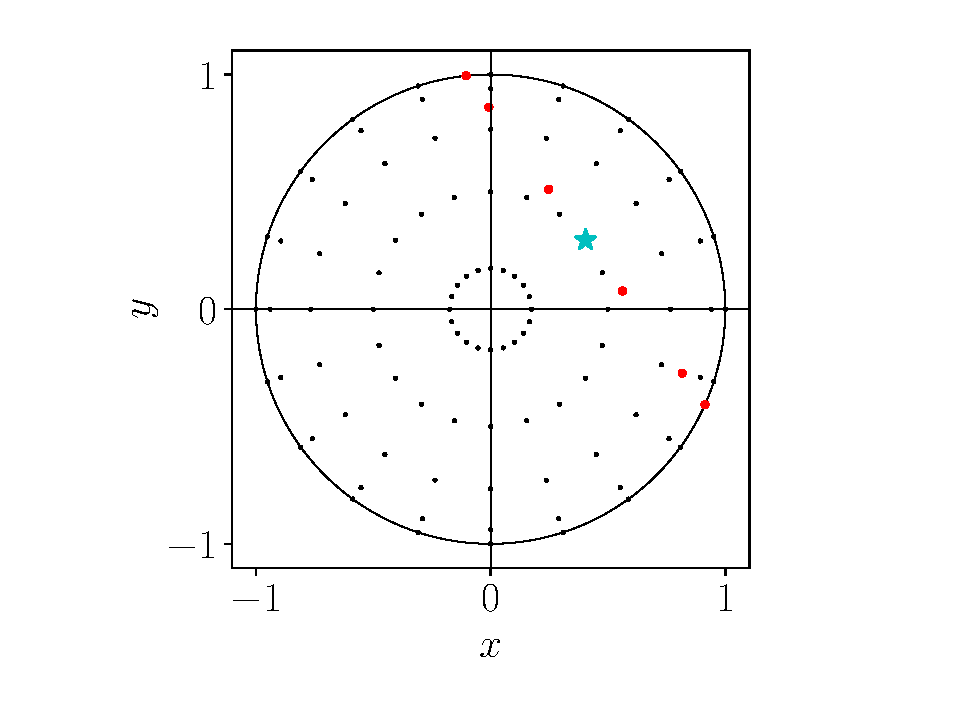
\includegraphics[scale=0.5]{figures/quad_5.pdf}
    \caption{6 point quadrature rule for the point $(x,y)$, denoted by a blue star.\\ Quadrature nodes labeled red, grid points labeled black}
\end{figure}
    
For the purposes of computing the proper inverse Radon transform, we perform the forward Radon transform as if we only know $f$ at the predefined grid points.
However, as shown in the figure above, these points rarely line up exactly with the points needed for quadrature.
Therefore, interpolation needs to be done to find those function values.
To obtain as much accuracy in the interpolation as possible, a series of one-dimensional interpolation schemes.
The point at which $f$ needs to be approximated is first projected onto the four closest diameters.
Barycentric interpolation is then performed along these diameters.
The stabilized barycentric interpolation formula \cite{Trefethen:7} is reproduced below.
\begin{align*}
    H_n(x)&= \frac{\sum_{j = 0}^{n} \alpha_j \frac{f_j}{x-x_j}}{\sum_{j = 0}^{n} \alpha_j\frac{1}{x-x_j}} \\ 
    \alpha_0 = \frac{1}{2},\quad \alpha_{1:n-1} = &(-1)^{1:n-1},\quad \alpha_n = \frac{1}{2} (-1)^n \\
\end{align*} 
Next, four point polynomial interpolation is performed across these four points.
Let $\theta_0$ be the midpoint of the arc containing $h_i$, $i=1,\dots,4$, obtained through barycentric interpolation:
\begin{align*}
    p(\theta) = - &\frac{1}{16}(h_1 - 9h_2 - 9h_3 + h_4) \\
    + &\frac{1}{24d\omega}(h_1 - 27h_2 + 27h_3 - h_4)(\theta - \theta_0) \\
    + &\frac{1}{4d\omega^2}(h_1 - h_2 - h_3 + h_4)(\theta - \theta_0)^2 \\
    - &\frac{1}{6d\omega^3}(h_1 - 3h_2 + 3h_3 - h_4)(\theta - \theta_0)^3
\end{align*}
\begin{figure}[H]
	\centering
	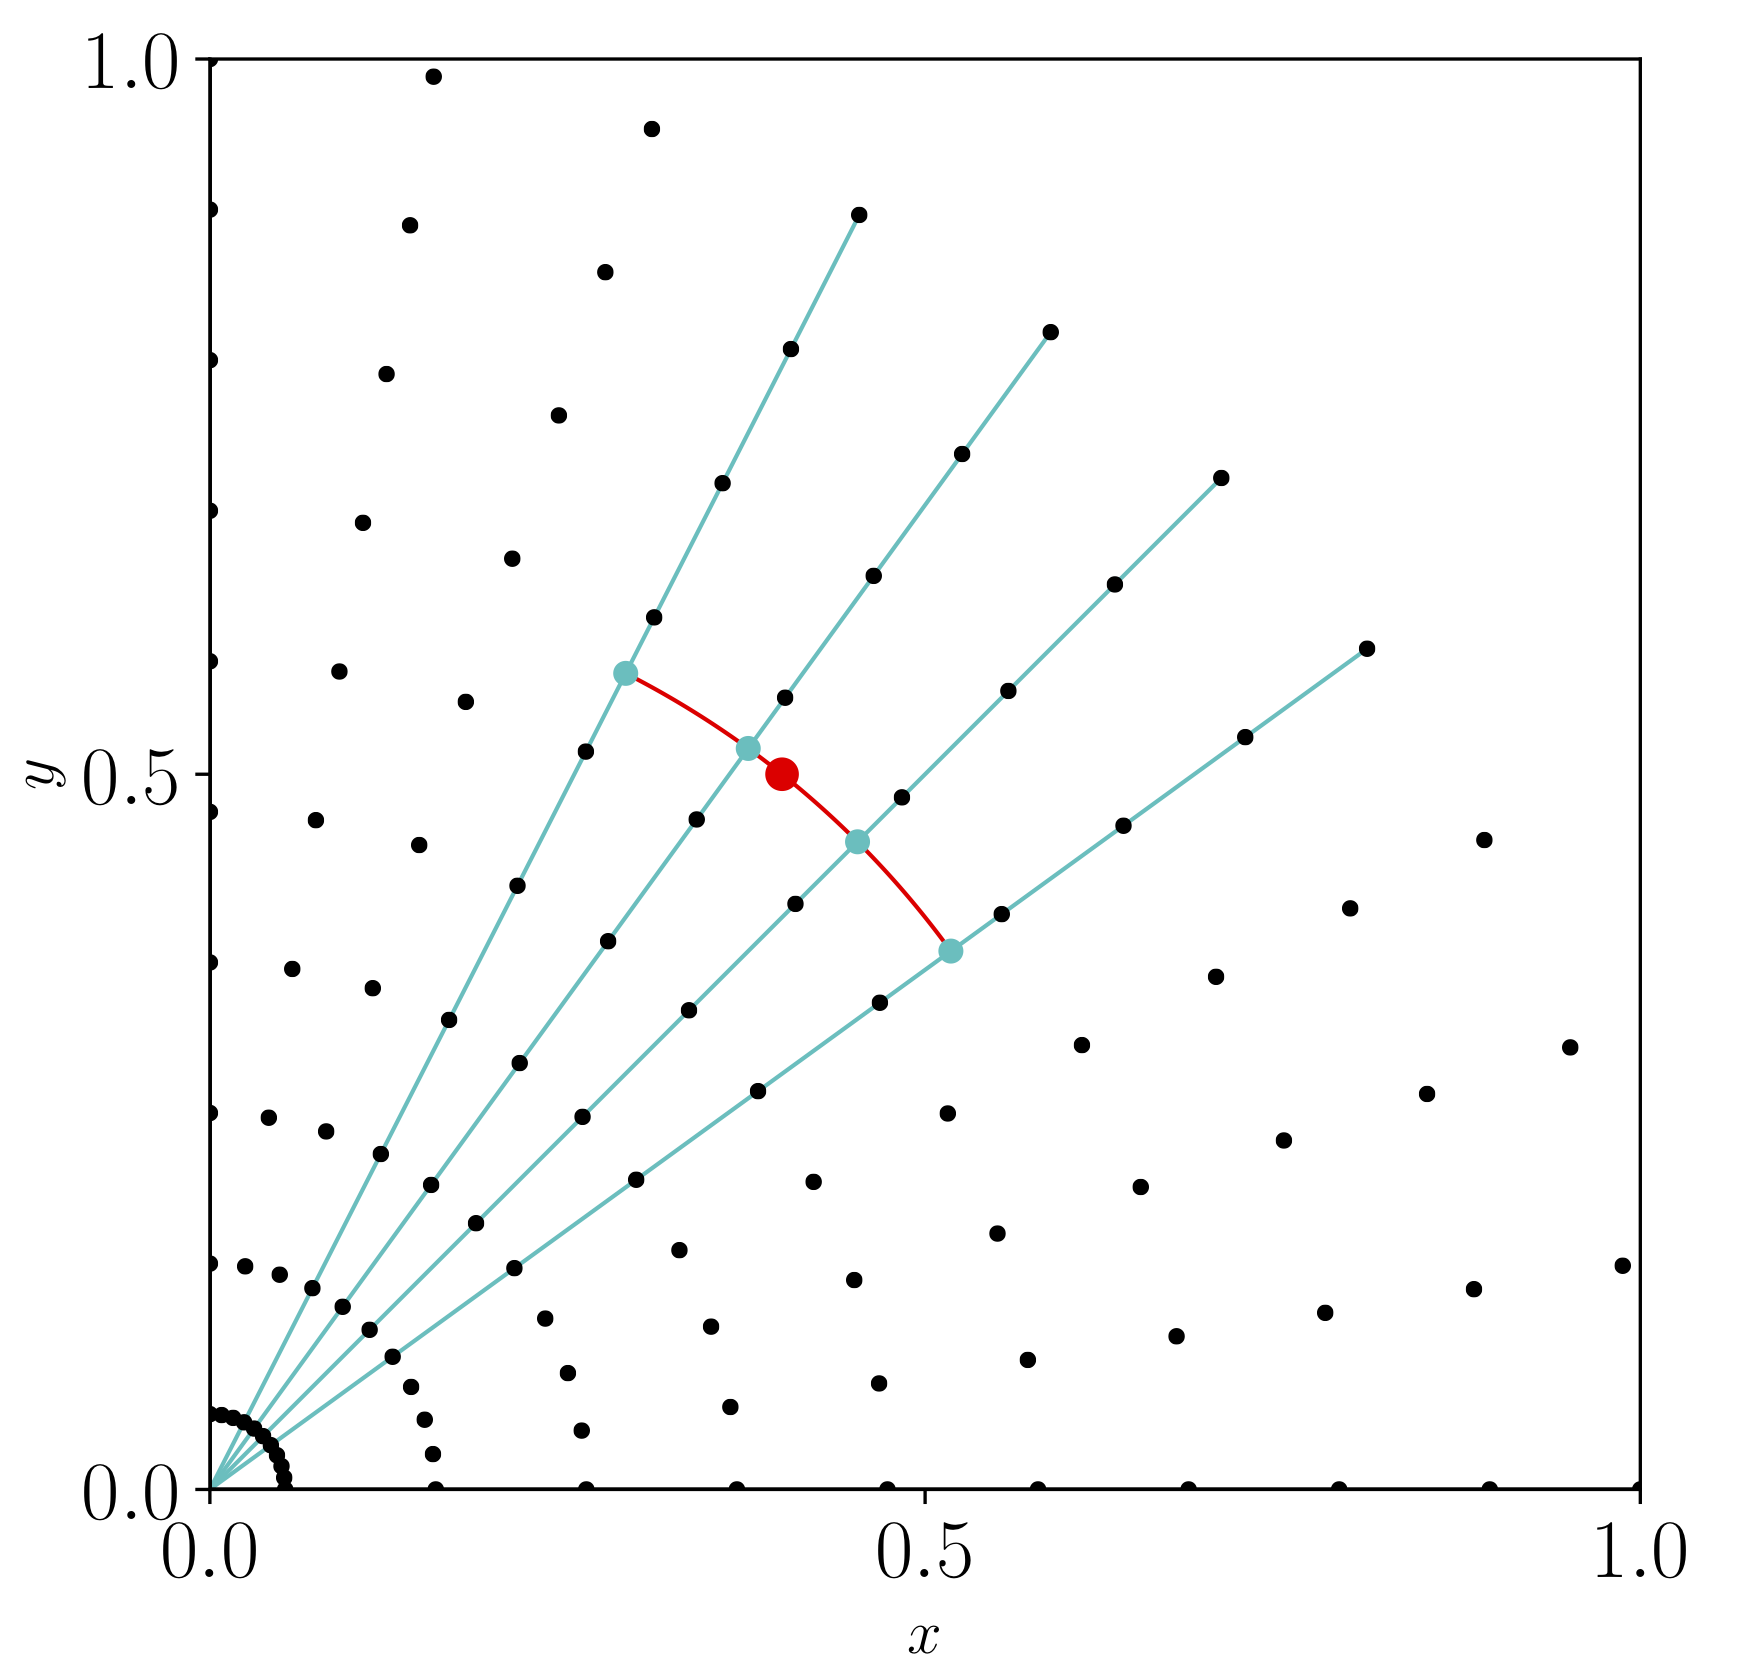
\includegraphics[scale=0.5]{figures/Interp4.png}
	\caption{Approximates $f$ at a point $(x, y)$, labeled with a red dot, \\using the values calculated at the four points labeled with a blue dot}
\end{figure}

This interpolation procedure is performed for each quadrature point for a single Radon transform evaluation.
The quadrature method itself is applied to each point in the grid, resulting in the Radon transform of our discretized domain.

\subsection{Backprojection}

The adjoint of the Radon transform, denoted $\mathcal{R}^{*}$, is known as \textbf{backprojection}. 
\par 
Given a function $\widehat{f}(s, \omega): \mathbb{R} \times \left[ 0, \pi \right] \rightarrow \mathbb{R}$, the backprojection of $\widehat{f}$ is defined as follows:
\begin{align*}
    \mathcal{R}^{*} \left( \widehat{f} \, \right) (x, y) := \int_{0}^{\pi} \widehat{f} \left( x \cos \left( \omega \right) + y \sin \left( \omega \right), \omega \right) \, d \omega
\end{align*}
Geometrically, the backprojection of $\widehat{f}$ at a point $\left( x, y \right)$ is the integral along the circle whose diameter is the line segment connecting $(x, y)$ and the origin.
\par 
The backprojection is useful in computing a stable inverse Radon transform \cite{Press:4}.

\subsection{Discretizing the Backprojection}

As was the case with the Radon transform, we need to discretize the backprojection for computational purposes.
Recall that our underlying mesh is parameterized by two integers:
\begin{itemize}
    \item $N_{\omega}$, the number of equi-spaced angles
    \item $N_{s}$, the number of Chebyshev points of the second kind along any one angle
\end{itemize}
This means our mesh consists of $N_{p} := N_{\omega} \times N_{s}$ points.
\par 
Given a function $\widehat{f} \left( s, \omega \right)$, we want to compute the \textit{approximate} backprojection $\widehat{f}$ at a mesh point $\left( x_{k}, y_{k} \right)$ where $k = 1, 2, \hdots, N_{p}$.
We can do this in the following manner:
\begin{enumerate}
    \item Draw a circle that passes through $\left( x_{k}, y_{k} \right)$ and the origin
    \item Select $N_{b}$ many equi-spaced (in angle) points along the circle's circumference
    \item Interpolate function values at the discrete points along the circle's circumference
    \item Use quadrature rules to approximate backprojection at $\left( x_{k}, y_{k} \right)$ using interpolated function values
\end{enumerate}
\textbf{Note:} We use the same four-point interpolation scheme discussed earlier to interpolate function values along the above circle.
\par 
The actual quadrature rule used in the above scheme is very simple.
Once we have interpolated $\widehat{f}$ at the $N_{b}$ many points, we simply take their sum and divide by $N_{b}$ to obtain the approximate backprojection of $\widehat{f}$ at $\left( x_{k}, y_{k} \right)$.
Just as in the Clenshaw-Curtis quadrature, this method is spectrally accurate.

\subsection{Inverse Radon Transform}

Recall that we have discretized the continuous Radon transform.
That is, we can approximate $\mathcal{R} \left( f \right) \left( s, \omega \right)$ on a mesh where
\begin{itemize}
    \item $f \left( x, y \right) : \mathbb{R}^{2} \rightarrow \mathbb{R}$ is a function with compact support on the unit disk, and 
    \item the mesh is parameterized by $N_{\omega}$ and $N_{s}$ and consists of $N_{p} := N_{\omega} \times N_{s}$ points
\end{itemize}
We typically have global knowledge of $f$, but as we have seen, we only use information about $f$ at the $N_p$ many mesh points to compute the approximate Radon transform of $f$ on the mesh.
\par 
That is, we only use $\vec{f} \in \mathbb{R}^{N_{p}}$ (a vector whose $i^{th}$ entry is $f$ evaluated at the $i^{th}$ mesh point) to compute $\widehat{\vec{f}} \in \mathbb{R}^{N_{p}}$ (a vector whose $i^{th}$ entry is an approximation of $\mathcal{R} \left( f \right)$ at the $i^{th}$ mesh point).
\par 
Concretely,
\begin{align}
    \mat{R} \, \vec{f} & = \widehat{\vec{f}}
\end{align}
where $\mat{R} \in \mathbb{R}^{N_{p} \times N_{p}}$ is a matrix whose $j^{th}$ column is the discretized Radon transform evaluated at $\vec{e_{j}} \in \mathbb{R}^{N_{p}}$, the $j^{th}$ canonical basis vector. 
\par 
%\textbf{Note:} We typically use a spectrally accurate method (rather than the fourth-order minimum method described earlier) to compute $\widehat{\vec{f}}$.
\par 
We are interested computing $\vec{f}$ given only $\widehat{\vec{f}}$.
Computationally, this is equivalent to solving $\mat{R} \, \vec{f} = \widehat{\vec{f}}$, which we try and solve with a number of direct and iterative solution techniques:
\begin{itemize}
    \item Gaussian elimination
    \item LU decompositions
    \item Row-action methods e.g. Kaczmarz's method
    \item Krylov subspace methods e.g. BiCGSTAB, GCRTOMK, etc.
\end{itemize}
However, the above system is \textit{highly} ill-conditioned and the above solvers yielded poor solutions.
\par 
We can try to alleviate this issue by applying a pre-conditioner to the system $\mat{R} \, \vec{f} = \widehat{\vec{f}}$, but there are several difficulties with this approach:
\begin{itemize}
    \item Pre-conditioners are typically selected on a case-by-case basis, and there does not appear to be much existing literature on how to select a pre-conditioner for this problem.
    \item Numerical tests show that $\mat{R}$ does not have ``nice" properties such as symmetry, positive (semi-)definiteness, etc.
    \item Numerical tests also show that $\mat{R}$ is not particularly sparse; as we increase the mesh resolution, the sparsity of $\mat{R}$ appears to asymptotically reach $\approx 50 \%$.
\end{itemize}
We investigated various pre-conditioners (despite the aforementioned difficulties) to see if they were feasible, including:
\begin{itemize}
    \item Sparse, incomplete LU (SPILU) decompositions
    \item Approximate pseudo-inverses 
\end{itemize}
However, these approaches did not fare much better.
Solving these pre-conditioned systems yielded better qualitative, but not better numerical, solutions.
\par 
Moreover, solving these pre-conditioned systems requires us to explicitly work with $\mat{R}$.
This is undesirable because $\mat{R}$ is expensive to compute (as we generate it column by column) and \textit{very} large.
\par 
However, note that 
\begin{align}
    \mat{R} \, \vec{f} = \widehat{\vec{f}} \quad \Longleftrightarrow \quad \mat{R}^{T} \, \mat{R} \, \vec{f} = \mat{R}^{T} \, \widehat{\vec{f}}
\end{align}
In this context, pre-multiplication by $\mat{R}^{T}$ means computing the approximate, discretized backprojection.
\par 
The system on the right is known as the \textbf{normal equations}, and there is one particular advantage to working with the normal equations compared to the system on the left.
Namely, $\mat{R}^{T} \, \mat{R}$ is symmetric, positive (semi-)definite.
This is useful if we choose to solve the normal equations via iterative methods that take advantage of this property e.g. the conjugate gradient method.
\par 
While we can generate $\mat{R}$ for a particular mesh and solve the normal equations $\mat{R}^{T} \, \mat{R} \, \vec{f} = \mat{R}^{T} \, \widehat{\vec{f}}$, this is not feasible for aforementioned reasons.
However, we do not need the matrix $\mat{R}^{T} \, \mat{R}$; we only need the matrix-vector products $\mat{R} \, \vec{f}$ and $\mat{R}^{T} \, \mat{R} \, \vec{f}$, which are far cheaper to compute.
\par 
\textbf{Note:} There is a caveat here. 
We have described ways of computing the approximate, discretized Radon transform and backprojection earlier, but computationally, they are \textbf{not} exact adjoints of one another.
This is due to the nature of our discretization scheme.
\par 
Since we only need knowledge of the matrix-vector products $\mat{R} \, \vec{f}$ and $\mat{R}^{T} \, \mat{R} \, \vec{f}$, we can solve the system
\begin{align}
    \mat{R}^{T} \, \mat{R} \, \vec{f} = \mat{R}^{T} \, \widehat{\vec{f}}
\end{align}
using iterative methods.
\par 
Here, the biconjugate gradient stabilized (BiCGSTAB) method was used to solve the above system with a starting guess of $\vec{f}^{(0)} = \vec{0}$.

% The \textbf{inverse Radon transform (IRT)} is an ill-posed problem. We want to solve $\mat{R}\,\vec{f} = \widehat{\vec{f}}$ for $\vec{f}$. However, $\mat{R}$ is nearly singular. Therefore, we were unable to solve using $\mat{R}^{-1}$. Fortunately, the following equations are equivalent.
% \begin{align*}
%     \mat{R} \, \vec{f} = \widehat{\vec{f}} \quad \Longleftrightarrow \quad \mat{R}^{T} \, \mat{R} \, \vec{f} = \mat{R}^{T} \, \widehat{\vec{f}}
% \end{align*}
% We are now able to perform the IRT.

% We use the BiCGSTAB iterative method to solve $\mat{R}^{T} \, \mat{R} \, \vec{f} = \mat{R}^{T} \, \widehat{\vec{f}}$. 